
 % or \
\chapter{Introduction}
\doublespacing
\label{chap:intro}
\minitoc
\section{Context: the rise of new content on the Web}

One of the significant changes of the Web during the 2000s was a move from Web 1.0 to Web 2.0. A main attribute of Web 2.0 is that it allows users to interact and collaborate with each other in a social media platform as creators of user-generated content\cite{moens2014mining} and members of (virtual) communities. In contrast, in Web 1.0 people are mostly limited to the passive viewing of content. Examples of Web 2.0 sites include social networking sites, blogs, forums, video, image or music sharing sites, etc. Web 2.0 does rely on this combination of contributing users and rich Web content. It is not limited to a network of relationship between users but rather built on the common interests shared among users. Therefore, when analyzing Web 2.0 structures and activities, it is crucial to jointly study both users and user-generated contents to really understand them. In other words, this analysis involves not only social network analysis (SNA) such as community detection or centrality calculation methods, but more generally social media mining techniques (e.g. Topic detection from user-generated content). Besides, users' behaviors and contributions are changing over time. So it is also important to consider a temporal dimension when performing such an analysis.


In parallel, the web also evolved from a Web of Documents to a Web augmented with Data readily available to software and machines. Following the W3C definition the "Semantic Web provides a common framework that allows data to be shared and reused across application, enterprise, and community boundaries".\footnote{\url{https://www.w3.org/2001/sw/} (accessed Feb 2016)}. However, most of the user-generated contents on the Web are unstructured and isolated except for some classical hyperlinks.


Apart from some pioneering initiatives \cite{chp1DBLP:journals/ijwbc/BreslinDHB06} \cite{chp1DBLP:journals/internet/BreslinD07} \cite{chp1DBLP:conf/webi/Mika04} \cite{chp1DBLP:conf/semweb/EreteoBGC09}  most of the user generated content does not benefit from the Linked Data of the Web and the models and formalisms of the Semantic Web. We need new methods and models in order to bridge social semantics and formal semantics on the Web \cite{gandon:hal-01059273}. In particular, it is essential to formalize these information and transform them into knowledge. 

In this thesis, we propose a framework, which combines social network analysis, social media mining and semantic web technologies, to help manage user-generated content websites. Figure \ref{fig:framework} shows an overview of the proposed framework discussed in this thesis.

\begin{figure}
\centering
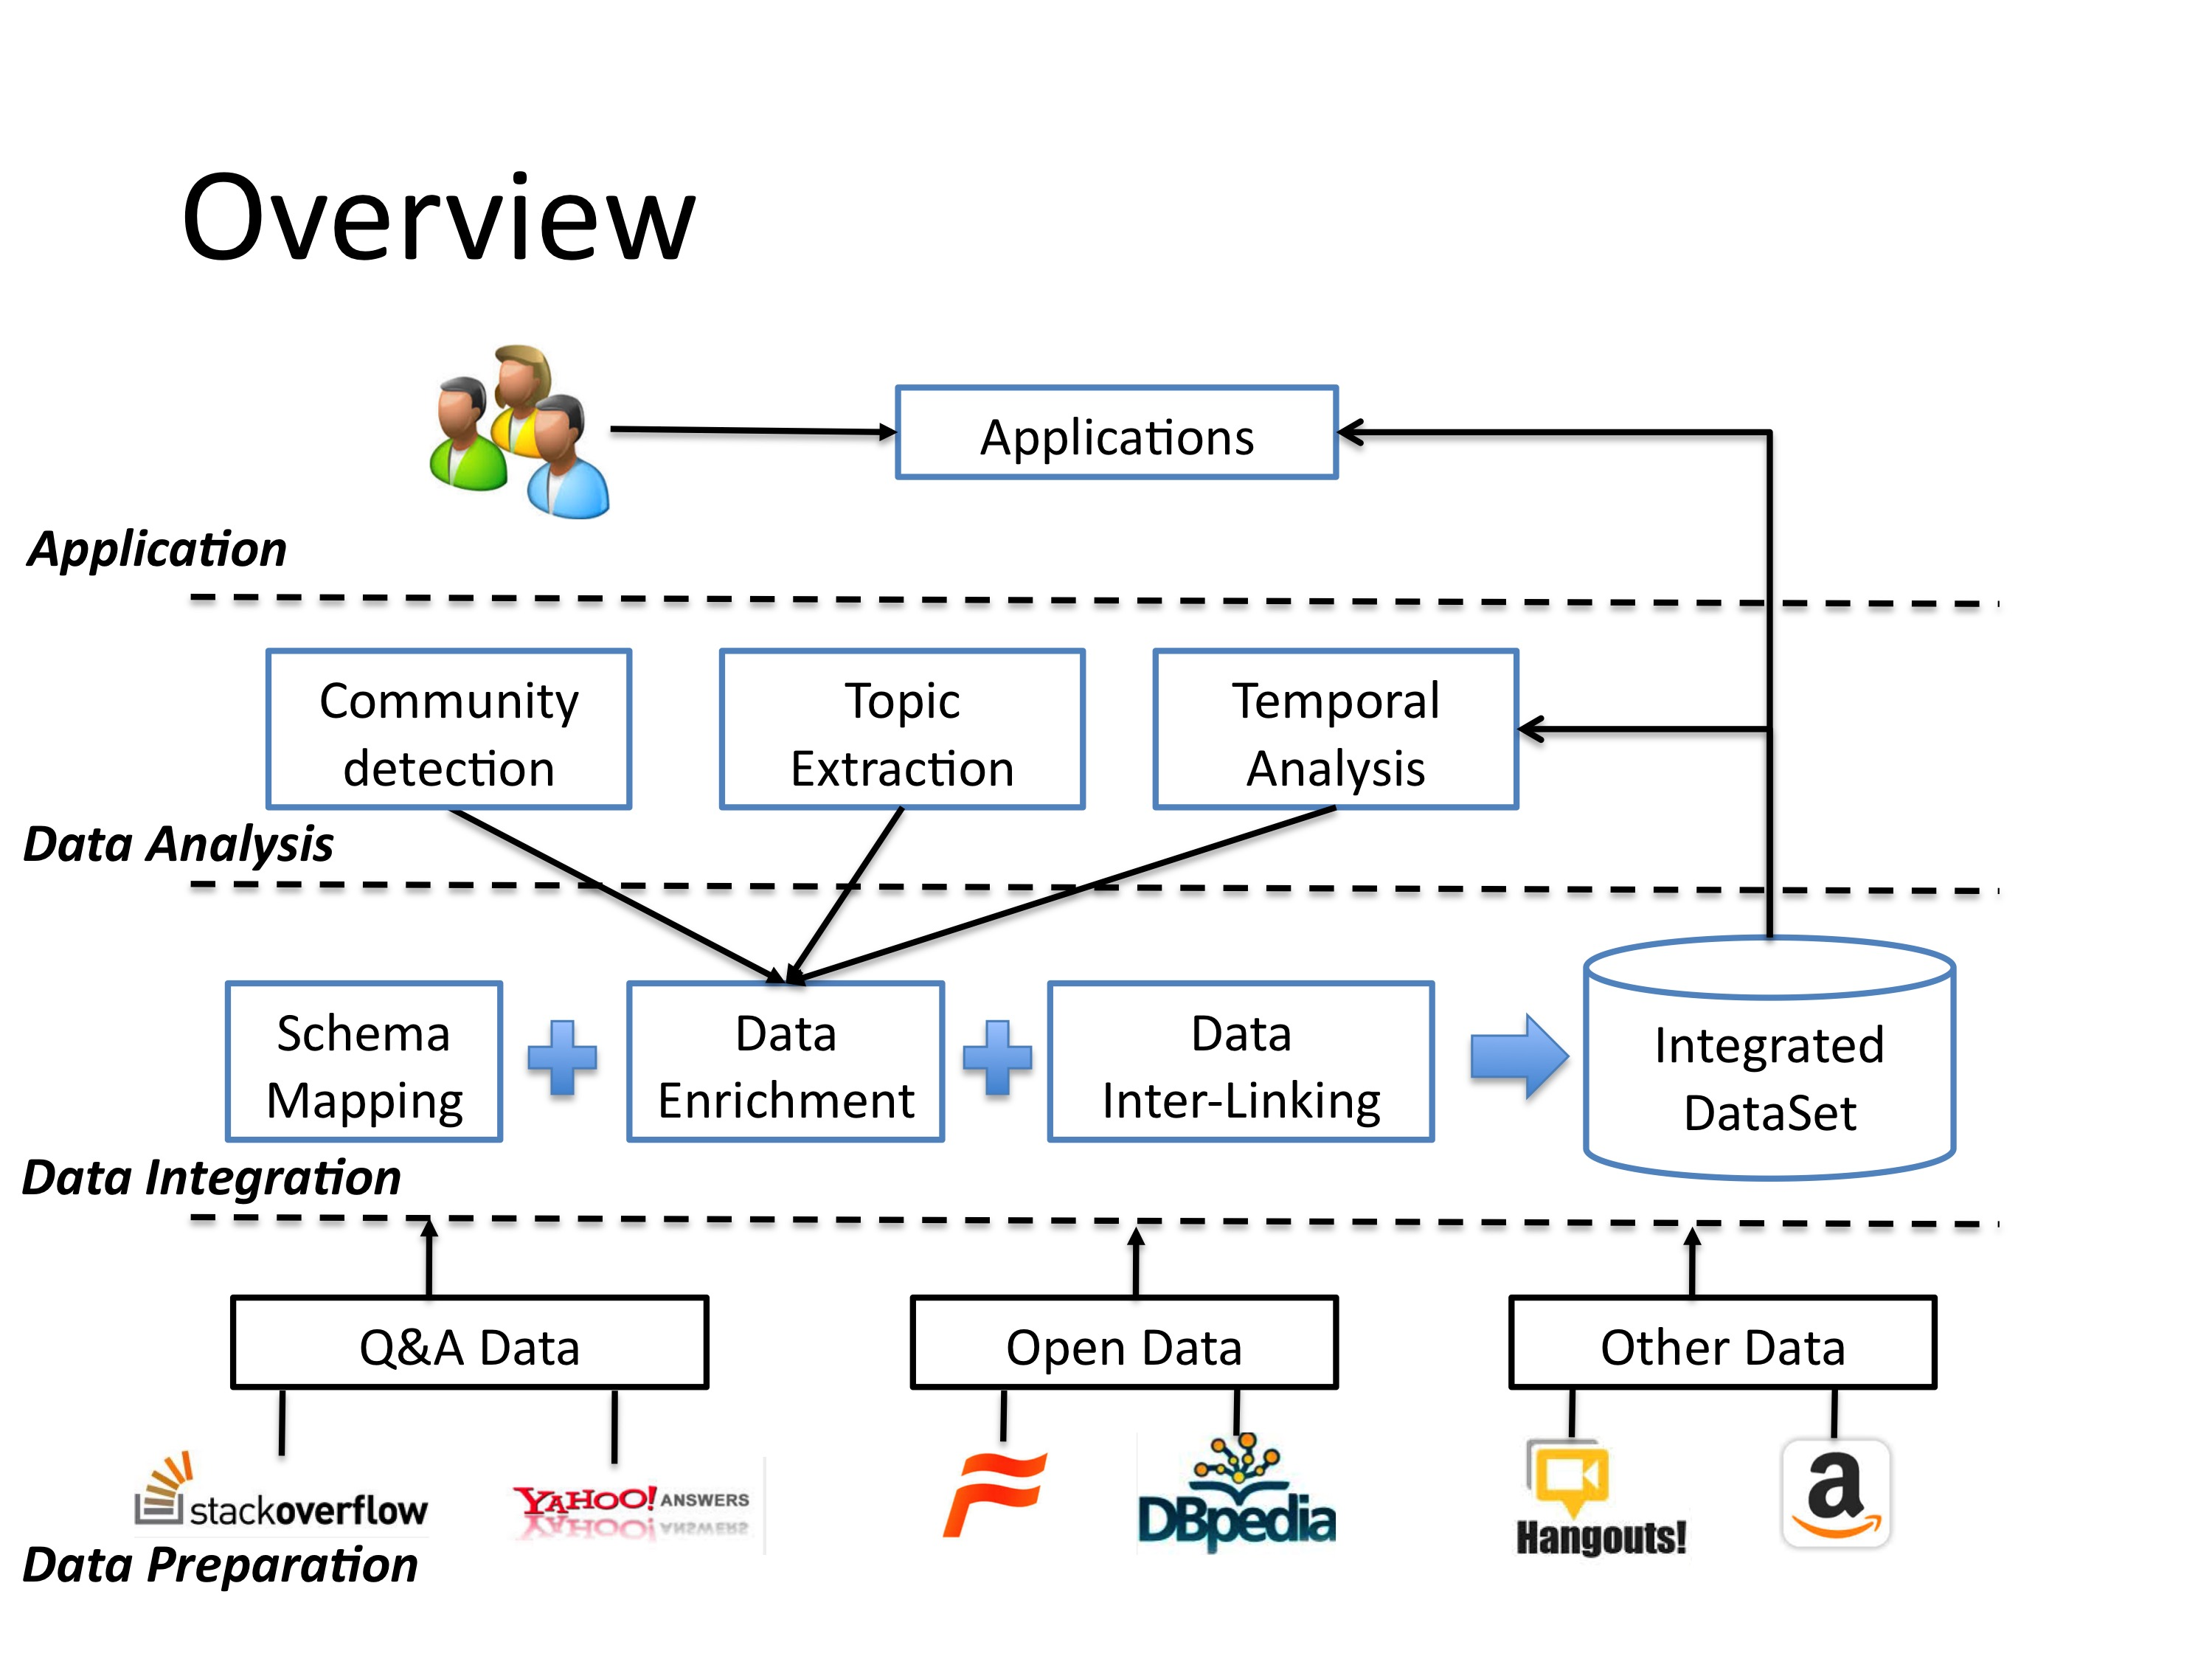
\includegraphics[width=5.5in]{framework.jpg}  
\caption{The overview of the framework proposed in this thesis to analyze Q\&A sites content and communities}
\label{fig:framework} 
\end{figure}



\section{Our Scenario: managing question-and-answer sites}


The main motivating scenario for this framework and our research questions is the case of question-and-answer sites (Q\&A sites), which is a very rich special case of user-generated content (UGC) website. Q\&A sites initially aimed at enabling users to ask questions to a community of experts. But since these exchanges are archived as Web pages they become user-generated Web content, formulated questions with submitted answers and comments, and they can be viewed and searched again later. So people with the same or similar questions can find answers by browsing or searching the questions that were already answered. On one hand, Q\&A sites rapidly became huge repositories of question-answer content supporting highly valuable and highly reusable knowledge~\cite{anderson2012discovering}. On the other hand, Q\&A sites also gather a large number of users who keep contributing questions and answers. Most of these users are more likely to ask questions on topics they are interested in, and to answer questions on topics they are experts of. So in addition to hosting a semi-structured content network, Q\&A sites have an implicit social structure and this is why Q\&A sites are particularly illustrative of the need to jointly study both users' social structures and user-generated contents as the two sides of the same coin.
Q\&A sites are also known as Community Question Answering (CQA), indicating the combination of the two key features of Q\&A sites: a community (the users) and questions and answers (the contents).


Tags and folksonomies gathering and organizing tags are quite common features in social networks, e.g. in Twitter \footnote{\url{https://twitter.com/} (accessed Feb 2016)}, del.icio.us \footnote{\url{http://delicious.com/} (accessed Feb 2016)}, Flickr \footnote{\url{ https://www.flickr.com/} (accessed Feb 2016)}, and also in some Q\&A sites such as StackOverflow\footnote{\url{http://stackoverflow.com/} (accessed Feb 2016)}.
They are a special case of user-generated content and the activity of associating tags to content is known as collaborative tagging or social bookmarking.   
Tags enable users to classify and find resources via shared tags; they can help creating communities, considering the fact that users sharing the same tags have common interests. Besides, tags can directly reflect users vocabulary and resources annotated with the same tags often are relative to the same topics. Therefore, finding communities and topics from tags is a key question. 
We will more specifically focus on the analysis of tags associated to questions and answers in CQA sites. 


Considering again the framework we propose, a first step is the design of schemas to formalize all of the meta-information we can export from a Q\&A site. Second, the resulting dataset can be analyzes in three different ways: social structure analysis, content analysis and evolution analysis. Then the results of these analysis will be integrated to the original dataset to enrich its structure and support new usages. Third, based on this integrated dataset, we will provide several social applications, such as question recommendation, expert detection and user life-cycle management. This is the basic logic of the proposed framework and in this thesis we will focus on the export and analysis stages, and in particular on overlapping community detection, shared interest labelling and temporal analysis.


The reason why we conduct three kinds of analysis is because we believe that they address three needs linked to the two main resources in Q\&A sites: the users' network and the Q\&A content. Indeed, from a user's perspective, detecting communities of interests is useful to reveal the sub-structures of the user network and identify relevant peers. More precisely, obtaining this information can contribute to the question routing problem~\cite{li2010routing}\cite{Zhou:2012:CAQ:2187980.2188201}, which is a very important Q\&A sites optimization problem, for example, to forward a question to a user who is active in the corresponding topic and has the expertise needed to answer it.
From the content's perspective, extracting topics is required to uncover the key subjects from massive content.
It is extremely useful for instance to retrieve already posted answers to a re-submitted question.
Moreover, both users and topics are changing over time, and therefore detecting such temporal dynamics is of prime importance to be aware of novelties. These indicators also are specially usefull to community managers; they can also contribute to the community management, for instance by allowing to track the interest evolution or community evolution in Q\&A sites.



\section{Research Question: topics, communities and trends in Q\&A sites}
In this section we summarize the main research questions that this thesis will address and answer.

\subsection*{RQ1. How to formalize user-generated content?}
The information in user-generated content is unstructured. A first issue is to formalize it. In addition, once an analysis has been performed, a second issue is to formalize the detected latent information and integrate it to the initial data in order to enrich it.

\subsection*{RQ2. How can we identify the common topics binding users together?}
On user-generated content websites, users  normally are creating information about their topics of interest. It is important to be able to detect these topics from the raw content generated by the users.

\subsection*{RQ3. How can we generate a semantic label for topics?}
Until now in our research questions we haven't characterized the representation of topics and in fact a topic consists mainly of a bag of words. One essential need is to automatically generate an adequate label for each topic to convey the meaning and coverage of the topic of shared interest it represents.

\subsection*{RQ4. How can we detect topic-based overlapping communities?}
We address the problem of overlapping community detection. Unlike traditional graph-structure based methods, we try to solve this problem by relying directly on topic modeling. The advantage is that detected topics can be directly used to interpret the \textit{raison d'être} of the communities. Another reason is that, regarding our scenario, Q\&A sites support social networking, however, unlike networks such as Facebook, there are no explicit relationship-based links between their users. In fact, Q\&A sites indirectly capture the connections made by users through the question-answer links or co-answer links. The users are neither mainly concerned with nor aware of the links existing between them. The social network is said to be implicit. Therefore, compared with other classical social networks, Q\&A networks contain more \textit{star-shape} structures (many users linked to a central user) than \textit{triangle-shape} structures (users linked to each other). As a result, many community detection algorithms developed to discover sub-structures in social networks do not apply to Q\&A implicit networks. 
Moreover, people may have multiple interests i.e. they may belong to several communities of interests. It is therefore important to be able to detect overlapping communities. 

\subsection*{RQ5. How can we extract topics-based expertise and temporal dynamics?}
The topics and the interest they attract change over time. We propose to address the problem of expert detection and temporal dynamics analysis together with topic modeling. 



\section{Contributions: models to identify shared interests and temporal dynamics}
The major contributions of this thesis are as follows.
\begin{itemize}
\item{To address the research question \textbf{RQ1}, we designed a prototype system to formalize both implicit and explicit information in question answer site, to extract the implicit information from the original explicit user-generated content, and to provide useful services by using these detected information. Besides, we proposed a vocabulary used to formalize the detected information.}

\item{To address the research question \textbf{RQ2}, we present a topic tree distribution method to extract topics from tags. We also propose a first-tag enrichment method to enrich questions which only have one or two tags. We show the effectiveness and efficiency of our topic extraction method.}

\item{To address the research question \textbf{RQ3}, we propose and compare metrics and provide a method using DBpedia to generate an adequate label for a bag of words capturing a topic.}

\item{To address the research question \textbf{RQ4}, based on our topic extraction method, we present a method to assign users to different topics in order to detect overlapping communities of interest.}

\item{To address the research question \textbf{RQ5}, we present a joint model to extract topic-based expertise and temporal dynamics from user-generated content. We also propose a post-processing method to model user activity. Traditionally, this information has been modeled separately.}

\end{itemize}



\section{Thesis Outline: social semantic Web and CQA sites mining}
This thesis contains a background and state of the art of related literature, an approach to detect topics from tags, an approach to detect overlapping communities and an approach to detect expertise and activities. The chapters in the rest of this thesis are organized as follows:
\begin{itemize}

\item{Chapter 2} provides a background of related domains, and the state of the art on community detection, topic modeling, expert detection and temporal analysis. We identify the research trends in the related areas, and outline the focus of this thesis.
\item{Chapter 3} describe QASM (Question \& Answer Social Media), a system based on social network analysis (SNA) to manage the two main resources in CQA sites: users and contents. We also present the QASM vocabulary used to formalize both the level of interest and the expertise of users on topics. 
\item{Chapter 4} describes an efficient approach for extracting data from Q\&A sites in order to detect communities of interest. We also present a method to enrich questions with a more general tag when they only have one or two tags. We then compare three detection methods we applied on a dataset extracted from the popular Q\&A site StackOverflow. Our method based on topic modeling and user membership assignment is shown to be much simpler and faster while preserving the quality of the detection. 
\item{Chapter 5} describes an approach to automatically generate a label for a topic by analyzing the meaning and links of its bag of words. We conduct a user study to compare different algorithms to choose the label.
\item{Chapter 6} describes a probabilistic graphical model to jointly model topics, expertises, activities and trends for a question answering Web application. We performed experiments with real-world data to confirm the effectiveness of our joint model, studying the users' behaviors and topics dynamics again on the dataset extracted from the popular question-answer site StackOverflow.
\item{Chapter 7} summarizes our contributions and describes our perspectives.
\end{itemize}



\section{Publications on the thesis contributions}
The publications resulting from this thesis are the following ones:

\begin{itemize}

\item{Journal} 


1. Zide Meng, Fabien L. Gandon, Catherine Faron-Zucker, Ge Song: Detecting topics and overlapping communities in question and answer sites. Social Network Analysis and Mining 5(1): 27:1-27:17 (2015)

2. Zide Meng, Fabien L. Gandon, Catherine Faron-Zucker: Overlapping Community Detection and Temporal Analysis on Q\&A Sites. Web Intelligence and Agent Systems 2016. 

\item{Conference Paper}

1. Zide Meng, Fabien L. Gandon, Catherine Faron-Zucker: Joint model of topics, expertises, activities and trends for question answering Web applications. IEEE/WIC/ACM Web Intelligence 2016.


2. Zide Meng, Fabien L. Gandon, Catherine Faron-Zucker: Simplified detection and labeling of overlapping communities of interest in question-and-answer sites. IEEE/WIC/ACM Web Intelligence 2015

3. Zide Meng, Fabien L. Gandon, Catherine Faron-Zucker, Ge Song: Empirical study on overlapping community detection in question and answer sites. IEEE/ACM ASONAM 2014: 344-348

4. Zide Meng, Fabien L. Gandon, Catherine Faron-Zucker: QASM: a Q\&A Social Media System Based on Social Semantic. International Semantic Web Conference (Posters \& Demos) 2014: 333-336

\end{itemize}
%\section*{backup information}






